\section{Introduzione}
\subsection{Obiettivo}
La presente relazione ha l'obiettivo di descrivere l'implementazione e l'analisi sperimentale delle \textit{statistiche d'ordine dinamiche}, realizzate in linguaggio \textit{Python} estendendo tre strutture dati distinte: una \textit{lista ordinata}, un \textit{albero binario di ricerca} (ABR) e un \textit{albero AVL}.

\medskip

L'obiettivo è confrontare le prestazioni delle tre implementazioni sottoponendole a test differenti, analizzando l'andamento ottenuto dei tempi di esecuzione e verificandone la coerenza con la complessità asintotica attesa dall'analisi teorica.

\subsection{Specifiche delle condizioni sperimentali}
Si riportano le specifiche hardware del calcolatore su cui sono stati svolti i test:
\begin{itemize}
	\item \textbf{CPU:} AMD Ryzen 5 5600H 6 core 12 threads
	\item \textbf{GPU:} AMD Radeon Graphics Vega 7 e NVIDIA GeForce RTX 3050
	\item \textbf{SSD:}	SSD M.2 PCIe NVMe 512 GB
	\item \textbf{RAM:} 16 GB DDR4-3200
	
\end{itemize}

Il codice è stato eseguito utilizzando \textbf{Python 3.14.4} e l'IDE \textbf{PyCharm 2026.1} su sistema operativo \textbf{Arch Linux}. La relazione è stata redatta utilizzando \TeX e \LaTeX e l'editor offline \textbf{TeXStudio v4.9.3}. Gli schemi UML sono stati realizzati utilizzando \textbf{mermaid.js}.

\newpage
\section{Fondamenti teorici}
\subsection{Statistiche d'ordine dinamiche}
Le statistiche d'ordine dinamiche sono delle particolari strutture dati aumentate che permettono di aggiungere due funzionalità principali:
\begin{itemize}
	\item \texttt{OS-SELECT(i)} che ritorna il puntatore al nodo con l'\textit{i-esima} chiave più piccola
	\item \texttt{OS-RANK(x)} che ritorna il rango di un determinato nodo a partire da un attraversamento ordinato
\end{itemize}

L'idea di base delle strutture dati aumentate consiste nel partire da una struttura esistente ed estenderla, ad esempio aggiungendo nuovi attributi ad ognuno dei suoi nodi, in modo da poter implementare in maniera efficiente nuovi metodi.\\
Nel caso specifico di questa relazione, ci interessa che sia possibile eseguire le operazioni di \textit{inserimento}, \textit{eliminazione}, \textit{ranking} e \textit{selezione}.

\subsection{Prestazioni attese}
Le prestazioni delle operazioni eseguite dipendono dalla struttura dati sottosotante e della scelte implementative adottate. Si prosegue andando ad analizzare ognuna delle implementazioni, analizzando nello specifico il caso peggiore, il caso medio e il caso peggiore.

\subsubsection*{Lista Ordinata}
Una lista ordinata è una struttura dati che mantiene i suoi elementi in ordine, in questo caso crescente. Il costo delle singole operazioni dipende dalla posizione dell'elemento su cui si vuole operare. Considerata una lita di $n$ elementi, si ha che nel caso migliore, l'operazione coinvolge solamente il primo elemento e si avrà quindi una complessità di $\Theta(1)$ mentre nel caso peggiore dovrò scorrere fino all'ultimo elemento e la complessità sarà dunque $\Theta(n)$. Per il caso medio si dovrà invece fare un'analisi probabilistica. Assumendo un input distribuito in maniera uniforme, il caso medio ci richiederà di scorrere circa $\frac{n}{2}$ elementi, risultando in una complessità di $O(n)$. \\
Per le specifiche operazioni si rimanda alla Tabella \ref{tab:complessita_lista_ordinata}.

\begin{table}[h!]
	\centering
\begin{tabular}{ |c||c|c|c|  }
	\hhline{~---}
	\multicolumn{1}{c|}{} & Caso peggiore & Caso medio & Caso migliore \\
	\hline
	Inserimento & $O(n)$ & $O(n)$ & $O(1)$\\
	\hline
	Eliminazione & $O(n)$ & $O(n)$ & $O(1)$\\
	\hline
	Ricerca & $\Theta(1)$ & $O(n)$ & $\Theta(n)$\\
	\hline
	Ranking & $O(n)$ & $O(n)$ & $O(1)$\\
	\hline
	Selezione & $\Theta(n)$ & $O(n)$ & $\Theta(1)$\\
	\hline
\end{tabular}
	\caption{Complessità lista ordinata}
	\label{tab:complessita_lista_ordinata}
\end{table}

\subsubsection*{Albero Binario di Ricerca}
Un albero binario di ricerca, comunemente abbreviato con ABR o dall'inglese BST, è una struttura costituita da nodi disposti in modo gerarchico. Ogni albero ha un nodo che svolge il ruolo di \textit{radice} (\textit{root}) e costituisce l'inizio della struttura. Poi ogni nodo presenta tre puntatori: uno al figlio destro, uno al figlio sinistro e uno al genitore. Ciò che caratterizza un ABR da altri tipi di alberi, è che l'unica regola di ordinamento è che la chiave (o il valore) del figlio sinistro di un nodo deve essere minore della chiave del nodo, mentre la chiave del figlio destro di nodo deve essere maggiore della chiave del nodo.\\
La complessità di un ABR dipende dunque dalla sua struttura interna e in particolare dalla sua altezza $h$, influenzata a sua volta dall'ordine di inserimento degli elementi.\\
Nel caso peggiore si avrà che il sottoalbero sinistro della radice contiene tutti gli $n$ elementi dell'albero, mentre il sottoalbero destro resta vuoto. In questo caso $h = n$. Nel caso migliore invece si avrà un albero perfettamente bilanciato in cui si può dimostrare che l'altezza è $h = \ln(n)$.\\
Per le specifiche operazioni si rimanda alla Tabella \ref{tab:complessita_albero_binario_ricerca}.

\begin{table}[h!]
	\centering
	\begin{tabular}{ |c||c|c|c|  }
		\hhline{~---}
		\multicolumn{1}{c|}{} & Caso peggiore & Caso medio & Caso migliore \\
		\hline
		Inserimento & $O(n)$ & $O(\ln(n))$ & $O(1)$\\
		\hline
		Eliminazione & $\Theta(1)$ & $O(n)$ & $\Theta(n)$\\
		\hline
		Ricerca & $\Theta(1)$ & $O(n)$ & $\Theta(n)$\\
		\hline
		Ranking & $\Theta(1)$ & $O(n)$ & $\Theta(n)$\\
		\hline
		Selezione & $\Theta(1)$ & $O(n)$ & $\Theta(n)$\\
		\hline
	\end{tabular}
	\caption{Complessità albero binario di ricerca}
	\label{tab:complessita_albero_binario_ricerca}
\end{table}

\subsubsection*{Albero AVL}
Un albero AVL è invece un albero quasi bilanciato, ovvero che per ogni nodo le altezze dei due sottoalberi destro e dinistro possono differire al massimo di un elemento. In questo tipo di albero si ha che l'altezza di un qualsiasi nodo è dato dal numero di archi nel cammino più lungo fino ad una estremità.
Essendo un albero sempre bilanciato si può dimostrare che l'altezza di un AVL che contiene $n$ nodi sarà $h \leq 2 \lg(n + 1)$. Tutte le operazioni che non modificano la struttura dell'albero hanno questa complessità.\\
Avendo questo vincolo sulle altezze, vengono aggiunti dei metodi chiamati di \textit{ristrutturazione} in particolare il \texttt{LEFT-ROTATE} per la rotazione a sinistra e il \texttt{RIGHT-ROTATE} per la rotazione a destra. Lo scopo di questi metodi è mantenere il \textit{Fattore di Bilanciamento}, o \textit{Balance Factor} $\leq 1$. \\
Per le specifiche operazioni si rimanda alla Tabella \ref{tab:complessita_albero_avl}.

\begin{table}[h!]
	\centering
	\begin{tabular}{ |c||c|c|c|  }
		\hhline{~---}
		\multicolumn{1}{c|}{} & Caso migliore & Caso medio & Caso peggiore \\
		\hline
		Inserimento & $O(n)$ & $O(h)$ & $\Theta(n)$\\
		\hline
		Eliminazione & $O(n)$ & $O(h)$ & $\Theta(n)$\\
		\hline
		Ricerca & $O(n)$ & $O(h)$ & $\Theta(n)$\\
		\hline
		Ranking & $\Theta(1)$ & $O(n)$ & $\Theta(n)$\\
		\hline
		Selezione & $\Theta(1)$ & $O(n)$ & $\Theta(n)$\\
		\hline
	\end{tabular}
	\caption{Complessità albero binario di ricerca}
	\label{tab:complessita_albero_avl}
\end{table}

\newpage

\section{Documentazione}
\subsection{Architettura del codice}
Il codice di laboratorio è diviso in tre parti principali: 
\begin{itemize}
	\item Implementazione delle strutture
	\item Implementazione dei test da effettuare
	\item Implementazione del plotter dei grafici
\end{itemize}


La parte di implementazione delle strutture include tre file principali, ognuno dei quali contiene due classi una per il nodo costituente e una per la struttura in sé. Il file \texttt{os\_orederd\_list.py} che comprende l'implementazione della statistica d'ordine dinamica con lista ordinata, \texttt{os\_bst.py} quella con l'albero binario di ricerca e \texttt{os\_avl.py} l'implementazione con l'albero AVL. \\

Il file \texttt{test\_runner.py} contiene l'implementazione di tutti quanti i test che devono essere effettuati. È qui che si trova la funzione \text{main()}.\\
Per finire troviamo il file \texttt{plot\_results.py} che si occupa del salvataggio e lettura dei dati grezzi in formato \texttt{.csv} oltre che al salvataggio di ogni singolo grafico in formato \texttt{.pdf}.


\subsection{Implementazione delle strutture dati}
Per il diagramma completo delle classi fare riferimento alla Figura \ref{fig:uml_implementazioni}.



\subsubsection*{Lista Ordinata}
Per l'implementazione tramite lista ordinata si crea una lista doppiamente collegata. Di fatto ogni \texttt{OrderedListNode} avrà tre attributi fondamentali: la chiave \texttt{key}, il puntatore al nodo successivo \texttt{next} e il puntatore al nodo precedente \texttt{prev}. Il nodo in testa alla lista avrà \texttt{prev}$= null$, mentre l'ultimo nodo della coda avrà \texttt{next}$= null$.

Di sotto si riporta la speigazione dei metodi della lista ordinata.
\begin{itemize}
	\item \texttt{insert(key)}: inserisce in maniera ordinata un nuovo elemento di chiave \texttt{key} nella lista.
	\item \texttt{delete(key)}: rimuove il primo elemento di chiave \texttt{key} dalla lista. Se l'elemento non è presente scorre tutta la lista. In seguito all'eleminazioni vengono aggiustati i puntatori dei nodi adiacenti a quello eliminato in maniera corretta.
	\item \texttt{print(key)}: scorre la lista e stampa ogni elemento in ordine.
	\item \texttt{select(i)}: restituisce la chiave dell'i-esimo nodo all'interno della lista
	\item \texttt{rank(key)}: restituisce la posizione a partire dalla testa della lista (rango) del nodo di chiave \texttt{key}.
\end{itemize} 

\subsubsection*{Albero Binario di Ricerca}
Il singolo nodo dell'ABR, \texttt{BSTNode} è stato implementato con gli attributi: la chiave \texttt{key}, il puntatore al figlio destro \texttt{right}, il puntatore al figlio sinistro \texttt{left} e il puntatore al padre \texttt{parent}. Il nodo radice \texttt{root} è l'unico che ha il puntatore \texttt{parent}$=null$.


Per l'albero bianrio di ricerca sono stati implementati i seguenti metodi:
\begin{itemize}
	\item \texttt{insert(key)}: inserisce l'emento di chiave $key$ all'interno dell'albero nella posizione corretta.
	\item \texttt{delete(key)}: rimuove l'elemento di chiave $key$ dall'albero effettuando in seguito una ristrutturazione per ricollegare i nodi in maniera corretta. Fa uso del metodo \texttt{successor(node)}.
	\item \texttt{print(key)}: metodo implementato per avere la stessa interfaccia fra le tre implementazioni. L'unica cosa che fa è chiamare il metodo \texttt{inorder\_tree\_walk()}.
	\item \sloppy \texttt{select(i)}: esplora l'albero e restituisce il nodo in posizione i-esima rispetto ad un \texttt{inorder\_tree\_walk()}.
	\item \texttt{rank(key)}: esplora l'albero e restituisce la posizione rispetto ad un \texttt{inorder\_tree\_walk()} del nodo di chiave \texttt{key}.
	\item \texttt{min(node)}: restituisce il nodo con la chiave più piccola. Per costruzione è il figlio più a sinistra.
	\item \texttt{max(node)}: restituisce il nodo con la chiave più grande. Per costruzione è il figlio più a destra.
	\item \texttt{find(node, key)}: cerca il nodo con la chiave \texttt{key}. Se non viene trovato restituisce $None$.
	\item \texttt{successor(node)}: restituisce il successore del nodo \textit{node}. Fa uso del metodo \texttt{min(node)}.
	\item \texttt{inorder\_tree\_walk(node)}: effettua un attraversamento ordinato dell'albero. Stampando gli elementi dal più piccolo al più grande.
	\item \texttt{size(node)}: Conta quanti nodi si trovano nei due sottoalberi destro e sinistro di \texttt{node}, compreso \texttt{node} stesso.
\end{itemize}

\subsubsection*{Albero AVL}
Il singolo nodo dell'Albero AVL, \texttt{AVLNode} è stato implementato con $5$ attributi: la chiave \texttt{key}, il puntatore al figlio destro \texttt{right}, il puntatore al figlio sinistro \texttt{left}, l'attributo \texttt{height} che tiene traccia del numero di archi nel percorso più lungo dal nodo alla foglia (primo nodo con entrambi i puntatori ai figli \textit{None}) e l'attributo size, che tiene traccia del numero totale di nodi nei sottoalberi destro e sinistro compreso il nodo radice. È l'analogo di \texttt{size(node)} dell'\textbf{ABR}, ma in questo caso invece di calcolarlo tutte le volte che mi serve, lo salvo come attributo e lo aggiorno solo quando modifico la struttura dell'albero.

Di sotto in dettaglio i metodi della classe:
\begin{itemize}
	\item \texttt{insert(key)}: inserisce l'emento di chiave \texttt{key} all'interno dell'albero nella posizione corretta. Effettua una rotazione appropriata per mantenere il \texttt{balance\_factor}$\leq 1$, utilizzando i metodi \texttt{right\_rotate(node)} e \texttt{left\_rotate(node)}.
	\item \texttt{delete(key)}: rimuove l'elemento di chiave \textit{key} dall'albero effettuando in seguito una ristrutturazione tramite rotazioni per bilanciare i nodi in maniera corretta. Fa uso del metodo \texttt{successor(node)}.
	\item \texttt{print(key)}: metodo implementato per avere la stessa interfaccia fra le tre implementazioni. L'unica cosa che fa è chiamare il metodo \texttt{inorder\_tree\_walk()}.
	\item \sloppy \texttt{select(i)}: esplora l'albero e restituisce il nodo in posizione i-esima rispetto ad un \texttt{inorder\_tree\_walk()}.
	\item \texttt{rank(key)}: esplora l'albero e restituisce la posizione rispetto ad un \texttt{inorder\_tree\_walk()} del nodo di chiave \texttt{key}.
	\item \texttt{get\_height(node)}: restituisce l'altezza del nodo \texttt{node}.
	\item \texttt{get\_size(node)}: restituisce la dimensione del nodo \texttt{node}.
	\item \texttt{get\_balance(node)}: restituisce il fattore di bilanciamento, \texttt{balance\_factor} del nodo \texttt{node}.
	\item \texttt{update(node)}: metodo di supporto. Ricalcola e aggiorna gli attributi \texttt{height} e \texttt{size} del nodo \texttt{node}.
	\item \texttt{right\_rotate(node)}: effettua una rotazione a destra dell'albero.
	\item \texttt{left\_rotate(nide)}: effettua una rotazione a sinistra dell'albero.
	\item \texttt{min(node)}: restituisce il nodo con la chiave più piccola. Per costruzione è il figlio più a sinistra.
	\item \texttt{max(node)}: restituisce il nodo con la chiave più grande. Per costruzione è il figlio più a destra.
	\item \texttt{successor(node)}: restituisce il successore del nodo \textit{node}. Fa uso del metodo \texttt{min(node)}.
	\item \texttt{inorder\_tree\_walk(node)}: effettua un attraversamento ordinato dell'albero. Stampando gli elementi dal più piccolo al più grande.
\end{itemize}

\begin{figure}[h]
	\centering
	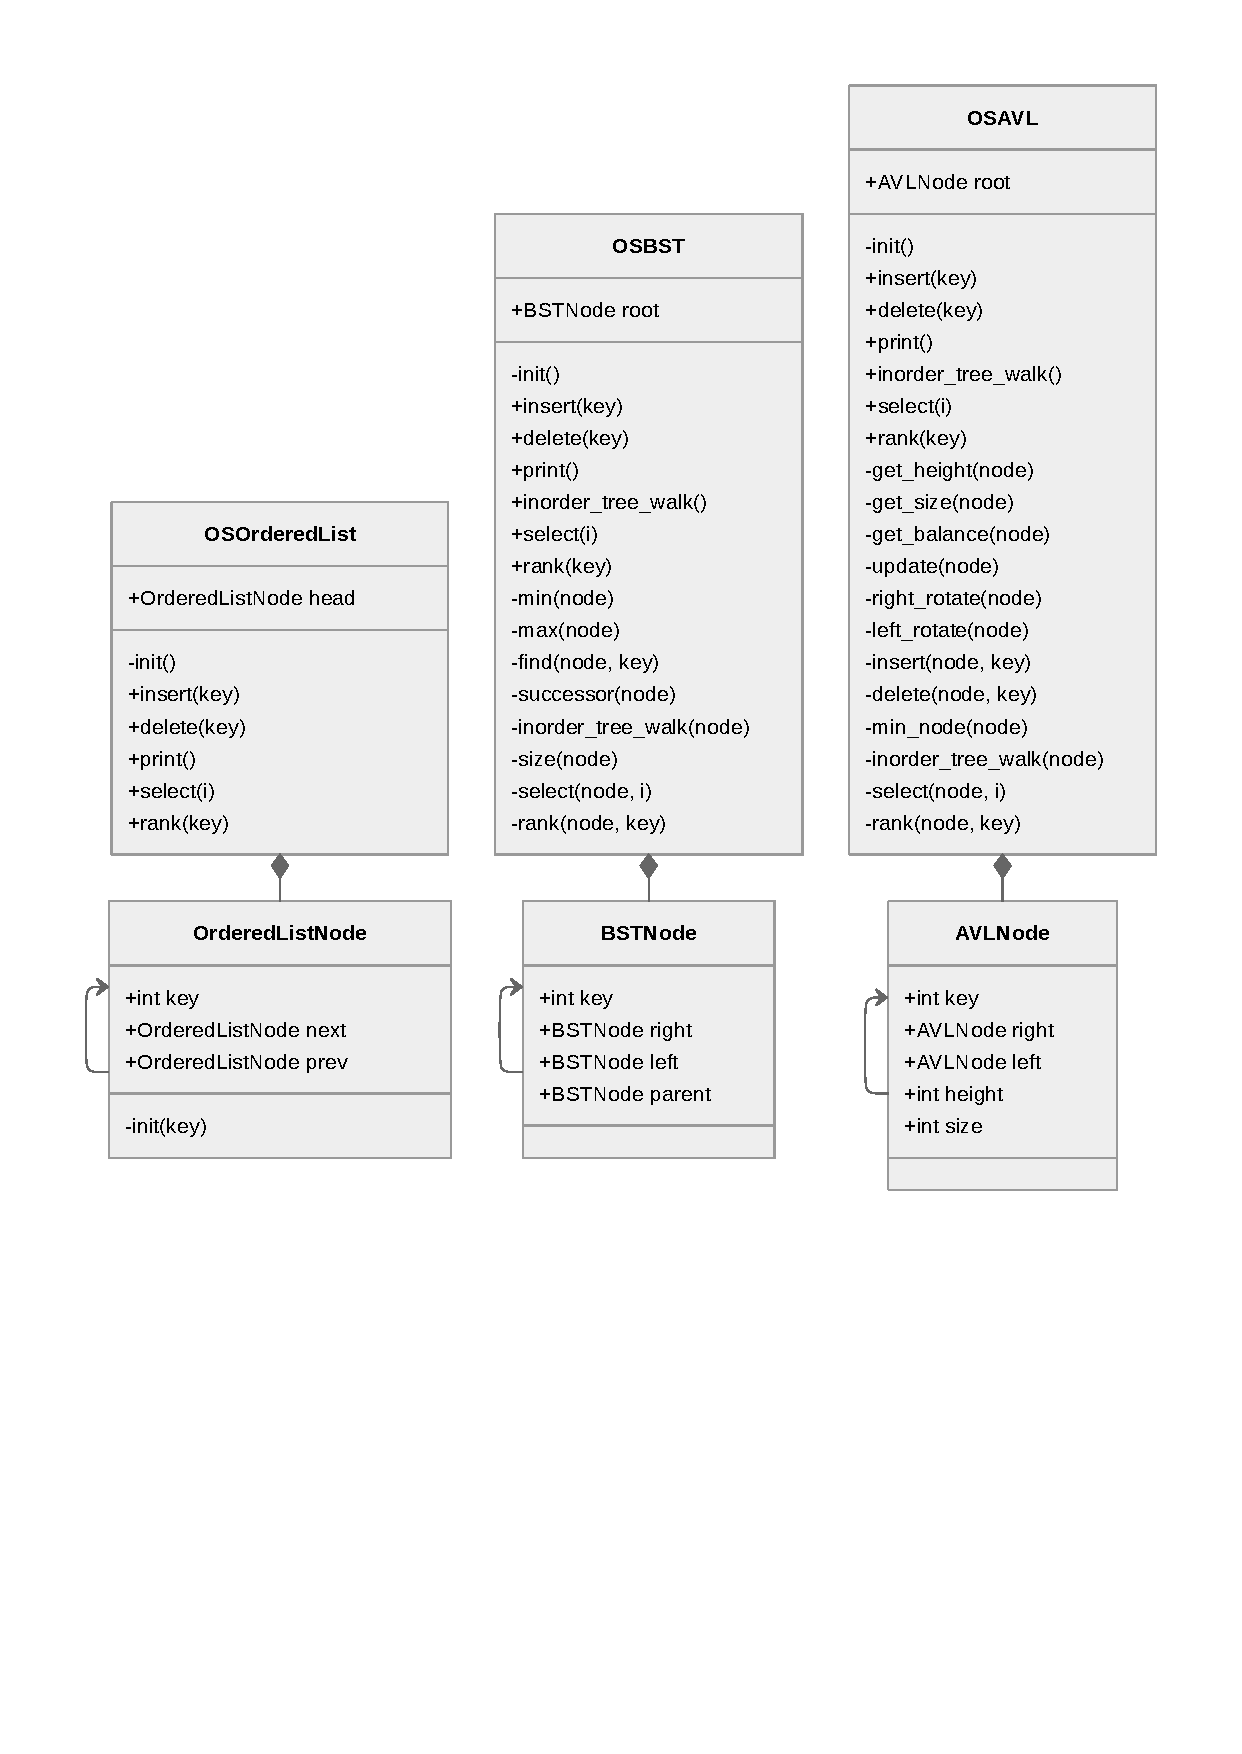
\includegraphics[width=1\textwidth]{figures/uml_implementazione_strutture.pdf}
	\caption{Diagramma UML delle tre implementazioni}
	\label{fig:uml_implementazioni}
\end{figure}

\clearpage

\subsection{Implementazione degli esperimenti}



\section{Esperimenti e risultati}
\subsection{Presentazione dei risultati}
\subsection{Analisi e discussione}

\section{Conclusioni}
